\newpage
\section{第一类方法:数据分布自适应}

数据分布自适应(Distribution Adaptation)是一类最常用的迁移学习方法。这种方法的基本思想是,由于源域和目标域的数据概率分布不同,那么最直接的方式就是通过一些变换,将不同的数据分布的距离拉近。

图~\ref{fig-distribution}形象地表示了几种数据分布的情况。\textit{简单来说,数据的边缘分布不同,就是数据整体不相似。数据的条件分布不同,就是数据整体相似,但是具体到每个类里,都不太相似。}

\begin{figure}[htbp]
	\centering
	\subfigure[源域数据]{
		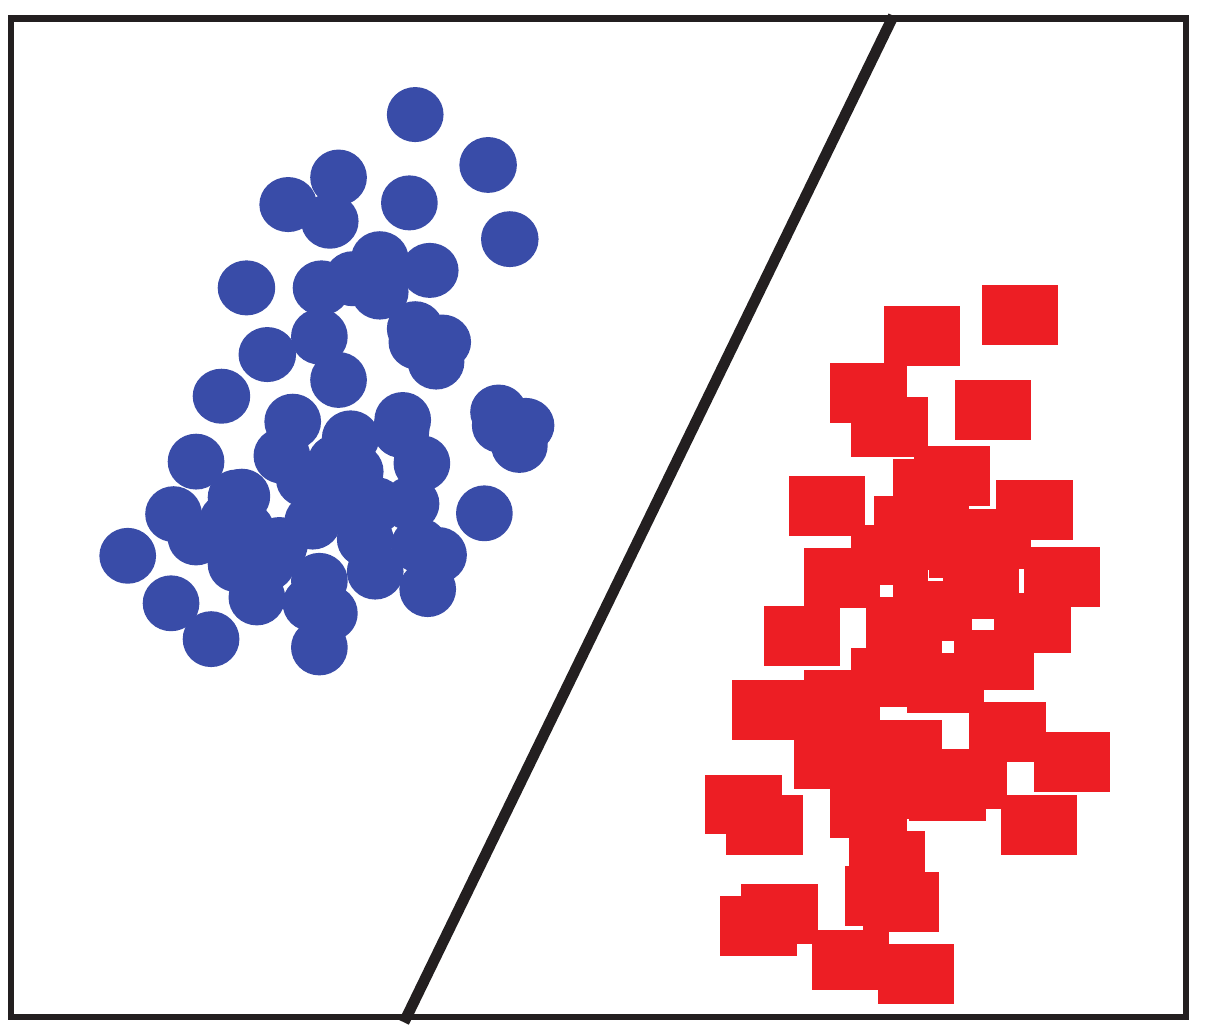
\includegraphics[scale=0.5]{./figures/fig-distribution-source.pdf}
		\label{fig-distribution-source}}
	~\vline
	~
	\subfigure[目标域数据: 类型I]{
		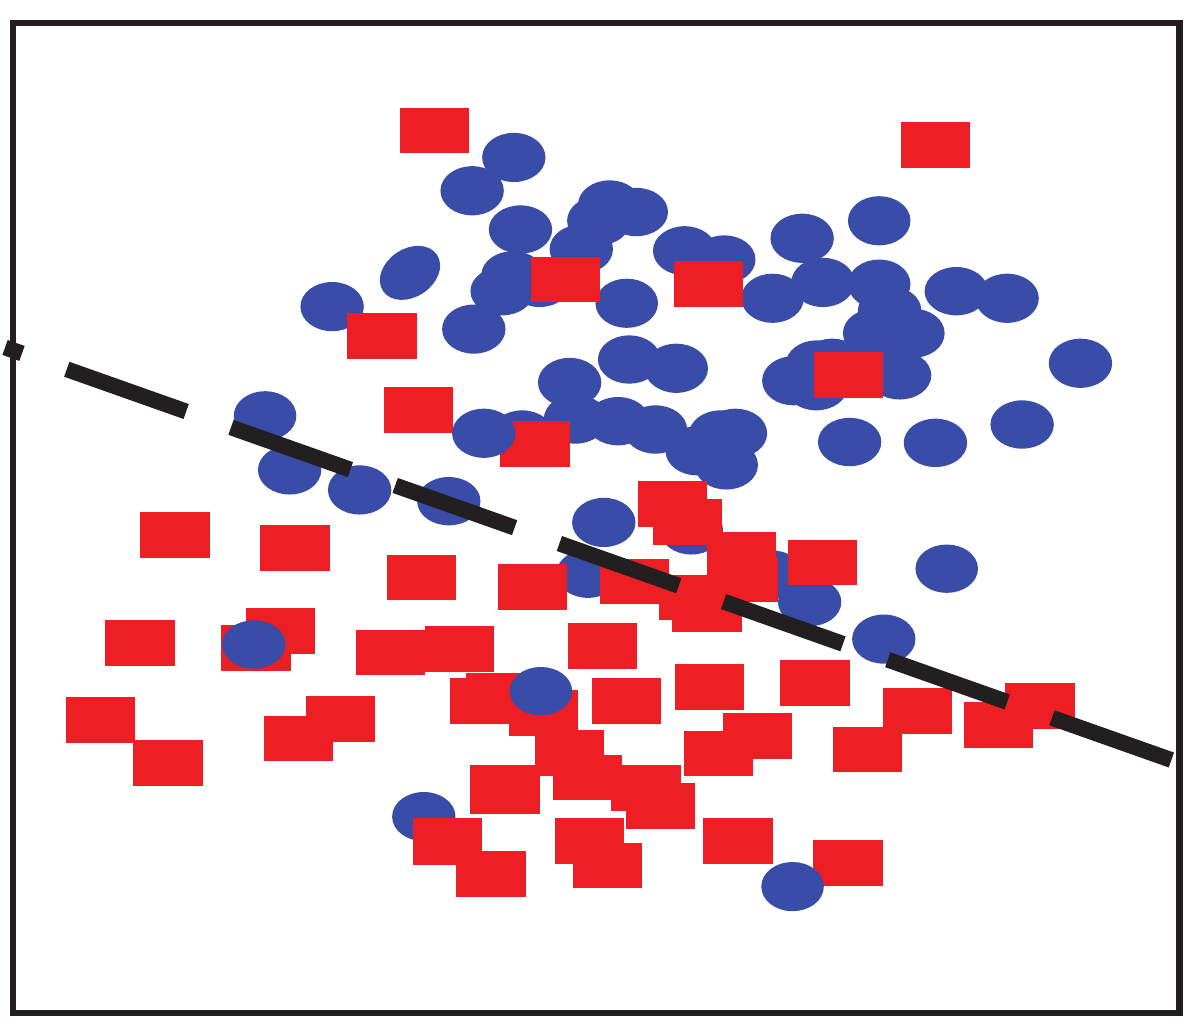
\includegraphics[scale=0.5]{./figures/fig-distribution-target1.pdf}
		\label{fig-distribution-target1}}
	~
	\subfigure[目标域数据:类型II]{
		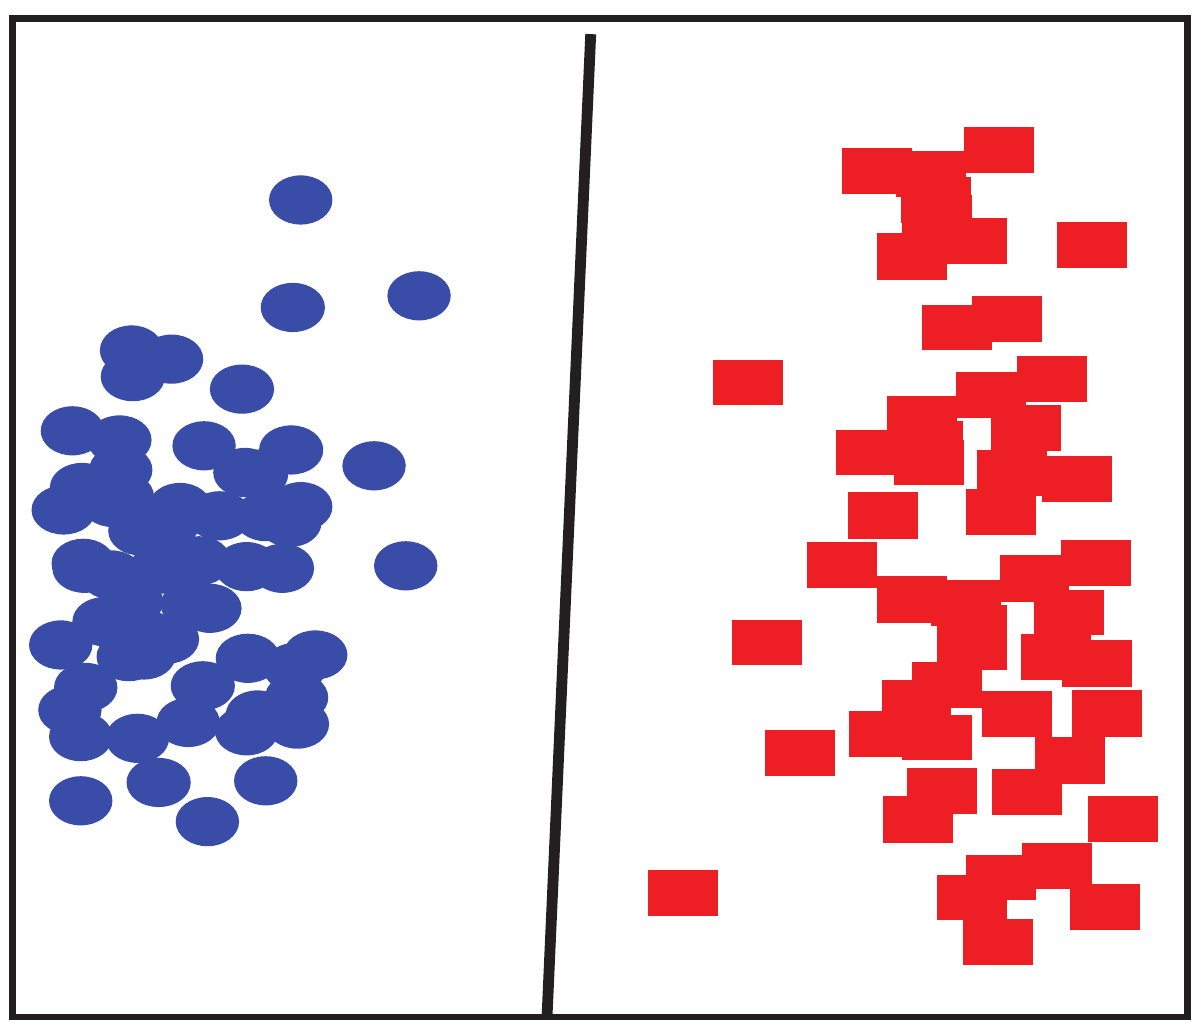
\includegraphics[scale=0.5]{./figures/fig-distribution-target2.pdf}
		\label{fig-distribution-target2}}
	\caption{不同数据分布的目标域数据}
	\label{fig-distribution}
\end{figure}

根据数据分布的性质,这类方法又可以分为\textit{边缘分布自适应、条件分布自适应}、以及\textit{联合分布自适应}。下面我们分别介绍每类方法的基本原理和代表性研究工作。介绍每类研究工作时,我们首先给出基本思路,然后介绍该类方法的核心,最后结合最近的相关工作介绍该类方法的扩展。

\subsection{边缘分布自适应}

\subsubsection{基本思路}

边缘分布自适应方法(Marginal Distribution Adaptation)的目标是减小源域和目标域的边缘概率分布的距离,从而完成迁移学习。从形式上来说,边缘分布自适应方法是用$P(\mathbf{x}_s)$和$P(\mathbf{x}_t)$之间的距离来近似两个领域之间的差异。即:

\begin{equation}
	\label{eq-marginal-general}
	DISTANCE(\mathcal{D}_s,\mathcal{D}_t) \approx ||P(\mathbf{x}_s) - P(\mathbf{x}_t)||
\end{equation}

边缘分布自适应对应于图~\ref{fig-distribution}中由图~\ref{fig-distribution-source}迁移到图~\ref{fig-distribution-target1}的情形。

\subsubsection{核心方法}

边缘分布自适应的方法最早由香港科技大学杨强教授团队提出~\cite{pan2011domain},方法名称为迁移成分分析(Transfer Component Analysis)。由于$P(\mathbf{x}_s) \ne P(\mathbf{x}_t)$,因此,直接减小二者之间的距离是不可行的。TCA假设存在一个特征映射$\phi$,使得映射后数据的分布$P(\phi(\mathbf{x}_s)) \approx P(\phi(\mathbf{x}_t))$。TCA假设如果边缘分布接近,那么两个领域的条件分布也会接近,即条件分布$P(y_s | \phi(\mathbf{x}_s))) \approx P(y_t | \phi(\mathbf{x}_t)))$。这就是TCA的全部思想。因此,我们现在的目标是,找到这个合适的$\phi$。

但是世界上有无穷个这样的$\phi$,也许终我们一生也无法找到合适的那一个。庄子说过,吾生也有涯,而知也无涯,以有涯随无涯,殆已!我们肯定不能通过穷举的方法来找$\phi$的。那么怎么办呢?

回到迁移学习的本质上来:最小化源域和目标域的距离。好了,我们能不能先假设这个$\phi$是已知的,然后去求距离,看看能推出什么呢?

更进一步,这个距离怎么算?机器学习中有很多种形式的距离,从欧氏距离到马氏距离,从曼哈顿距离到余弦相似度,我们需要什么距离呢?TCA利用了一个经典的也算是比较“高端”的距离叫做最大均值差异(MMD,maximum mean discrepancy)。我们令$n_1,n_2$分别表示源域和目标域的样本个数,那么它们之间的MMD距离可以计算为:

\begin{equation}
	\label{eq-distribution-mmd}
	DISTANCE(\mathbf{x}_{s},\mathbf{x}_{t})= \begin{Vmatrix} \frac{1}{n_1} \sum \limits_{i=1}^{n_1} \phi(\mathbf{x}_{i}) - \frac{1}{n_2}\sum \limits _{j=1}^{n_2} \phi(\mathbf{x}_{j}) \end{Vmatrix}_{\mathcal{H}}
\end{equation}

MMD是做了一件什么事呢?简单,就是求映射后源域和目标域的\textit{均值之差}。

事情到这里似乎也没什么进展:我们想求的$\phi$仍然没法求。

TCA是怎么做的呢,这里就要感谢矩阵了!我们发现,上面这个MMD距离平方展开后,有二次项乘积的部分!那么,联系在SVM中学过的核函数,把一个难求的映射以核函数的形式来求,不就可以了?于是,TCA引入了一个核矩阵$\mathbf{K}$:

\begin{equation}
	\mathbf{K}=\begin{bmatrix}\mathbf{K}_{s,s} & \mathbf{K}_{s,t}\\\mathbf{K}_{t,s} & \mathbf{K}_{t,t}\end{bmatrix} 
\end{equation}

以及一个MMD矩阵$\mathbf{L}$,它的每个元素的计算方式为:

\begin{equation}
	l_{ij}=\begin{cases} \frac{1}{{n_1}^2} & \mathbf{x}_i,\mathbf{x}_j \in \mathcal{D}_s,\\ \frac{1}{{n_2}^2} & \mathbf{x}_i,\mathbf{x}_j \in \mathcal{D}_t,\\ -\frac{1}{n_1 n_2} & \text{otherwise} \end{cases}
\end{equation}

这样的好处是,直接把那个难求的距离,变换成了下面的形式:

\begin{equation}
	\mathrm{tr}(\mathbf{KL})-\lambda \mathrm{tr}(\mathbf{K})
\end{equation}

其中,$\mathrm{tr}(\cdot)$操作表示求矩阵的迹,用人话来说就是一个矩阵对角线元素的和。这样是不是感觉离目标又进了一步呢?

其实这个问题到这里就已经是可解的了,也就是说,属于计算机的部分已经做完了。只不过它是一个数学中的半定规划(SDP,semi-definite programming)的问题,解决起来非常耗费时间。由于TCA的第一作者Sinno Jialin Pan以前是中山大学的数学硕士,他想用更简单的方法来解决。他是怎么做的呢?

他想出了用降维的方法去构造结果。用一个更低维度的矩阵$\mathbf{W}$:
\begin{equation}
	\widetilde{\mathbf{K}}=({\mathbf{K}}{\mathbf{K}}^{-1/2}\widetilde{\mathbf{W}})(\widetilde{\mathbf{W}}^{\top}{\mathbf{K}}^{-1/2}{\mathbf{K}})={\mathbf{K}}\mathbf{W} \mathbf{W}^{\top}{\mathbf{K}}
\end{equation}

这里的$\mathbf{W}$矩阵是比$\mathbf{K}$更低维度的矩阵。最后的$\mathbf{W}$就是问题的解答了!

好了,问题到这里,整理一下,TCA最后的优化目标是:

\begin{equation}
	\begin{split} \min_\mathbf{W} \quad& \mathrm{tr}(\mathbf{W}^\top \mathbf{K} \mathbf{L} \mathbf{K} \mathbf{W}) + \mu \mathrm{tr}(\mathbf{W}^\top \mathbf{W})\\ \text{s.t.} \quad & \mathbf{W}^\top \mathbf{K} \mathbf{H} \mathbf{K} \mathbf{W} = \mathbf{I}_m \end{split} 
\end{equation}

这里的$\mathbf{H}$是一个中心矩阵,$\mathbf{H} = \mathbf{I}_{n_1 + n_2} - 1/(n_1 + n_2)\mathbf{11}^\top$.

这个式子下面的条件是什么意思呢?那个$\min$的目标我们大概理解,就是要最小化源域和目标域的距离,加上$\mathbf{W}$的约束让它不能太复杂。那么下面的条件是什么呢?下面的条件就是要实现第二个目标:维持各自的数据特征。

TCA要维持的是什么特征呢?文章中说是variance,但是实际是scatter matrix,就是数据的散度。就是说,一个矩阵散度怎么计算?对于一个矩阵$\mathbf{A}$,它的scatter matrix就是$\mathbf{A} \mathbf{H} \mathbf{A}^\top$。这个$\mathbf{H}$就是上面的中心矩阵啦。

解决上面的优化问题时,作者又求了它的拉格朗日对偶。最后得出结论,$\mathbf{W}$的解就是它的前$m$个特征值!简单不?数学美不美?

好了,我们现在总结一下TCA方法的步骤。输入是两个特征矩阵,我们首先计算$\mathbf{L}$和$\mathbf{H}$矩阵,然后选择一些常用的核函数进行映射(比如线性核、高斯核)计算$\mathbf{K}$,接着求$({\mathbf{K}} \mathbf{L} {\mathbf{K}}+\mu \mathbf{I})^{-1}{\mathbf{K}} \mathbf{H}{\mathbf{K}}$的前$m$个特征值。仅此而已。然后,得到的就是源域和目标域的降维后的数据,我们就可以在上面用传统机器学习方法了。

为了形象地展示TCA方法的优势,我们借用~\cite{pan2011domain}中提供的可视化效果,在图中展示了对于源域和目标域数据(红色和蓝色),分别由PCA(主成分分析)和TCA得到的分布结果。从图~\ref{fig-distribution-tca}中可以很明显地看出,对于概率分布不同的两部分数据,在经过TCA处理后,概率分布更加接近。这说明了TCA在拉近数据分布距离上的优势。

\begin{figure}[htbp]
	\centering
	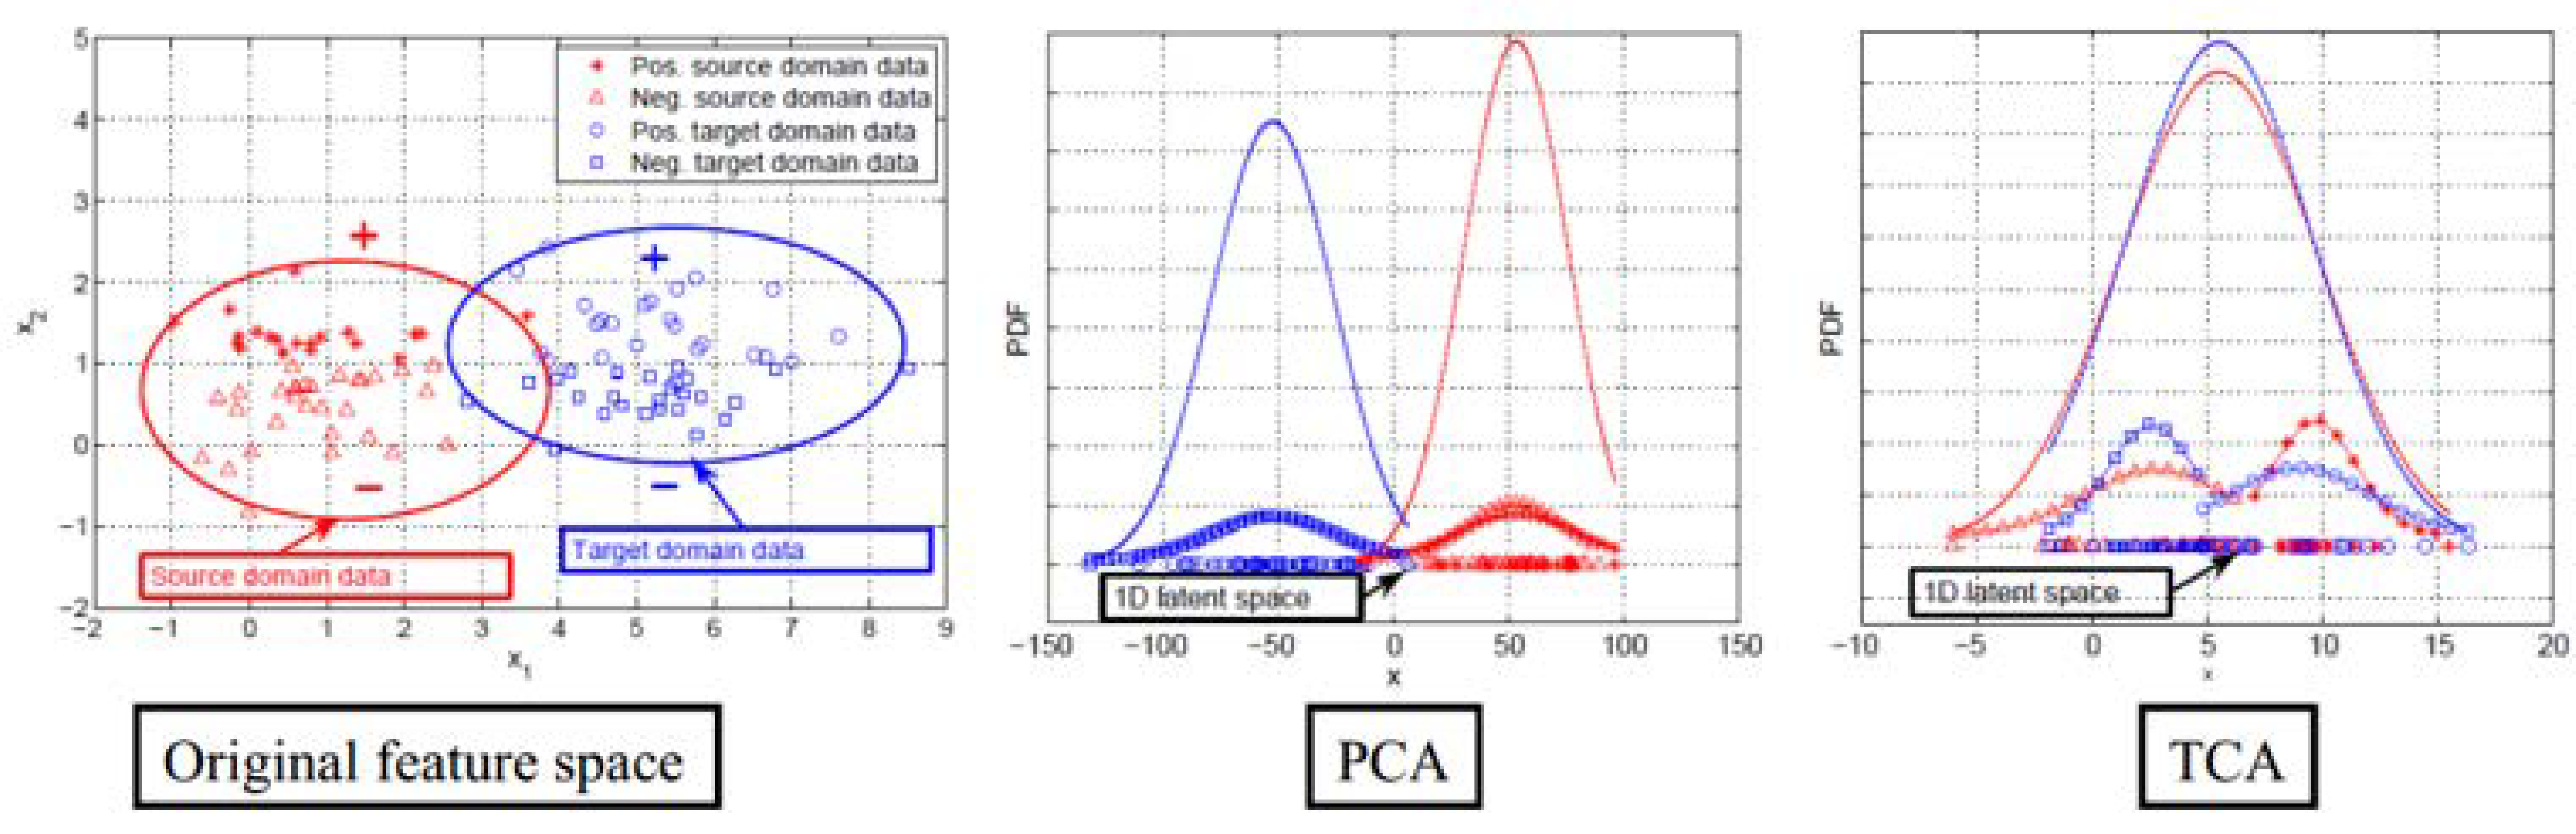
\includegraphics[scale=0.6]{./figures/fig-distribution-tca.pdf}
	\caption{TCA和PCA的效果对比}
	\label{fig-distribution-tca}
\end{figure}

\subsubsection{扩展}

TCA方法是迁移学习领域一个经典的方法,之后的许多研究工作都以TCA为基础。我们列举部分如下:

\begin{itemize}
	\item ACA (Adapting Component Analysis)~\cite{dorri2012adapting}: 在TCA中加入HSIC
	\item DTMKL (Domain Transfer Multiple Kernel Learning)~\cite{duan2012domain}: 在TCA中加入了MK-MMD,用了新的求解方式
	\item TJM (Transfer Joint Matching)~\cite{long2014transfer}: 在优化目标中同时进行边缘分布自适应和源域样本选择
	\item DDC (Deep Domain Confusion)~\cite{tzeng2014deep}: 将MMD度量加入了深度网络特征层的loss中(我们将会在深度迁移学习中介绍此工作)
	\item DAN (Deep Adaptation Network)~\cite{long2015learning}: 扩展了DDC的工作,将MMD换成了MK-MMD,并且进行多层loss计算(我们将会在深度迁移学习中介绍此工作)
	\item DME (Distribution Matching Embedding): 先计算变换矩阵,再进行特征映射(与TCA顺序相反)
	\item CMD (Central Moment Matching)~\cite{zellinger2017central}: MMD着眼于一阶,此工作将MMD推广到了多阶
\end{itemize}

\subsection{条件分布自适应}

条件分布自适应方法(Conditional Distribution Adaptation)的目标是减小源域和目标域的条件概率分布的距离,从而完成迁移学习。从形式上来说,条件分布自适应方法是用$P(y_s|\mathbf{x}_s)$和$P(y_t|\mathbf{x}_t)$之间的距离来近似两个领域之间的差异。即:

\begin{equation}
\label{eq-conditional-general}
DISTANCE(\mathcal{D}_s,\mathcal{D}_t) \approx ||P(y_s|\mathbf{x}_s) - P(y_t|\mathbf{x}_t)||
\end{equation}

条件分布自适应对应于图~\ref{fig-distribution}中由图~\ref{fig-distribution-source}迁移到图~\ref{fig-distribution-target2}的情形。

目前单独利用条件分布自适应的工作较少,这些工作主要可以在~\cite{saito2017asymmetric}中找到。最近,中科院计算所的Wang等人提出了STL方法(Stratified Transfer Learning)~\cite{wang2018stratified}。作者提出了\textit{类内迁移}(Intra-class Transfer)的思想。指出现有的绝大多数方法都只是学习一个全局的特征变换(Global Domain Shift),而忽略了类内的相似性。类内迁移可以利用类内特征,实现更好的迁移效果。

STL方法的基本思路如图~\ref{fig-distribution-stl}所示。首先利用大多数投票的思想,对无标定的位置行为生成伪标签;然后在再生核希尔伯特空间中,利用类内相关性进行自适应地空间降维,使得不同情境中的行为数据之间的相关性增大;最后,通过二次标定,实现对未知标定数据的精准标定。

\begin{figure}[htbp]
	\centering
	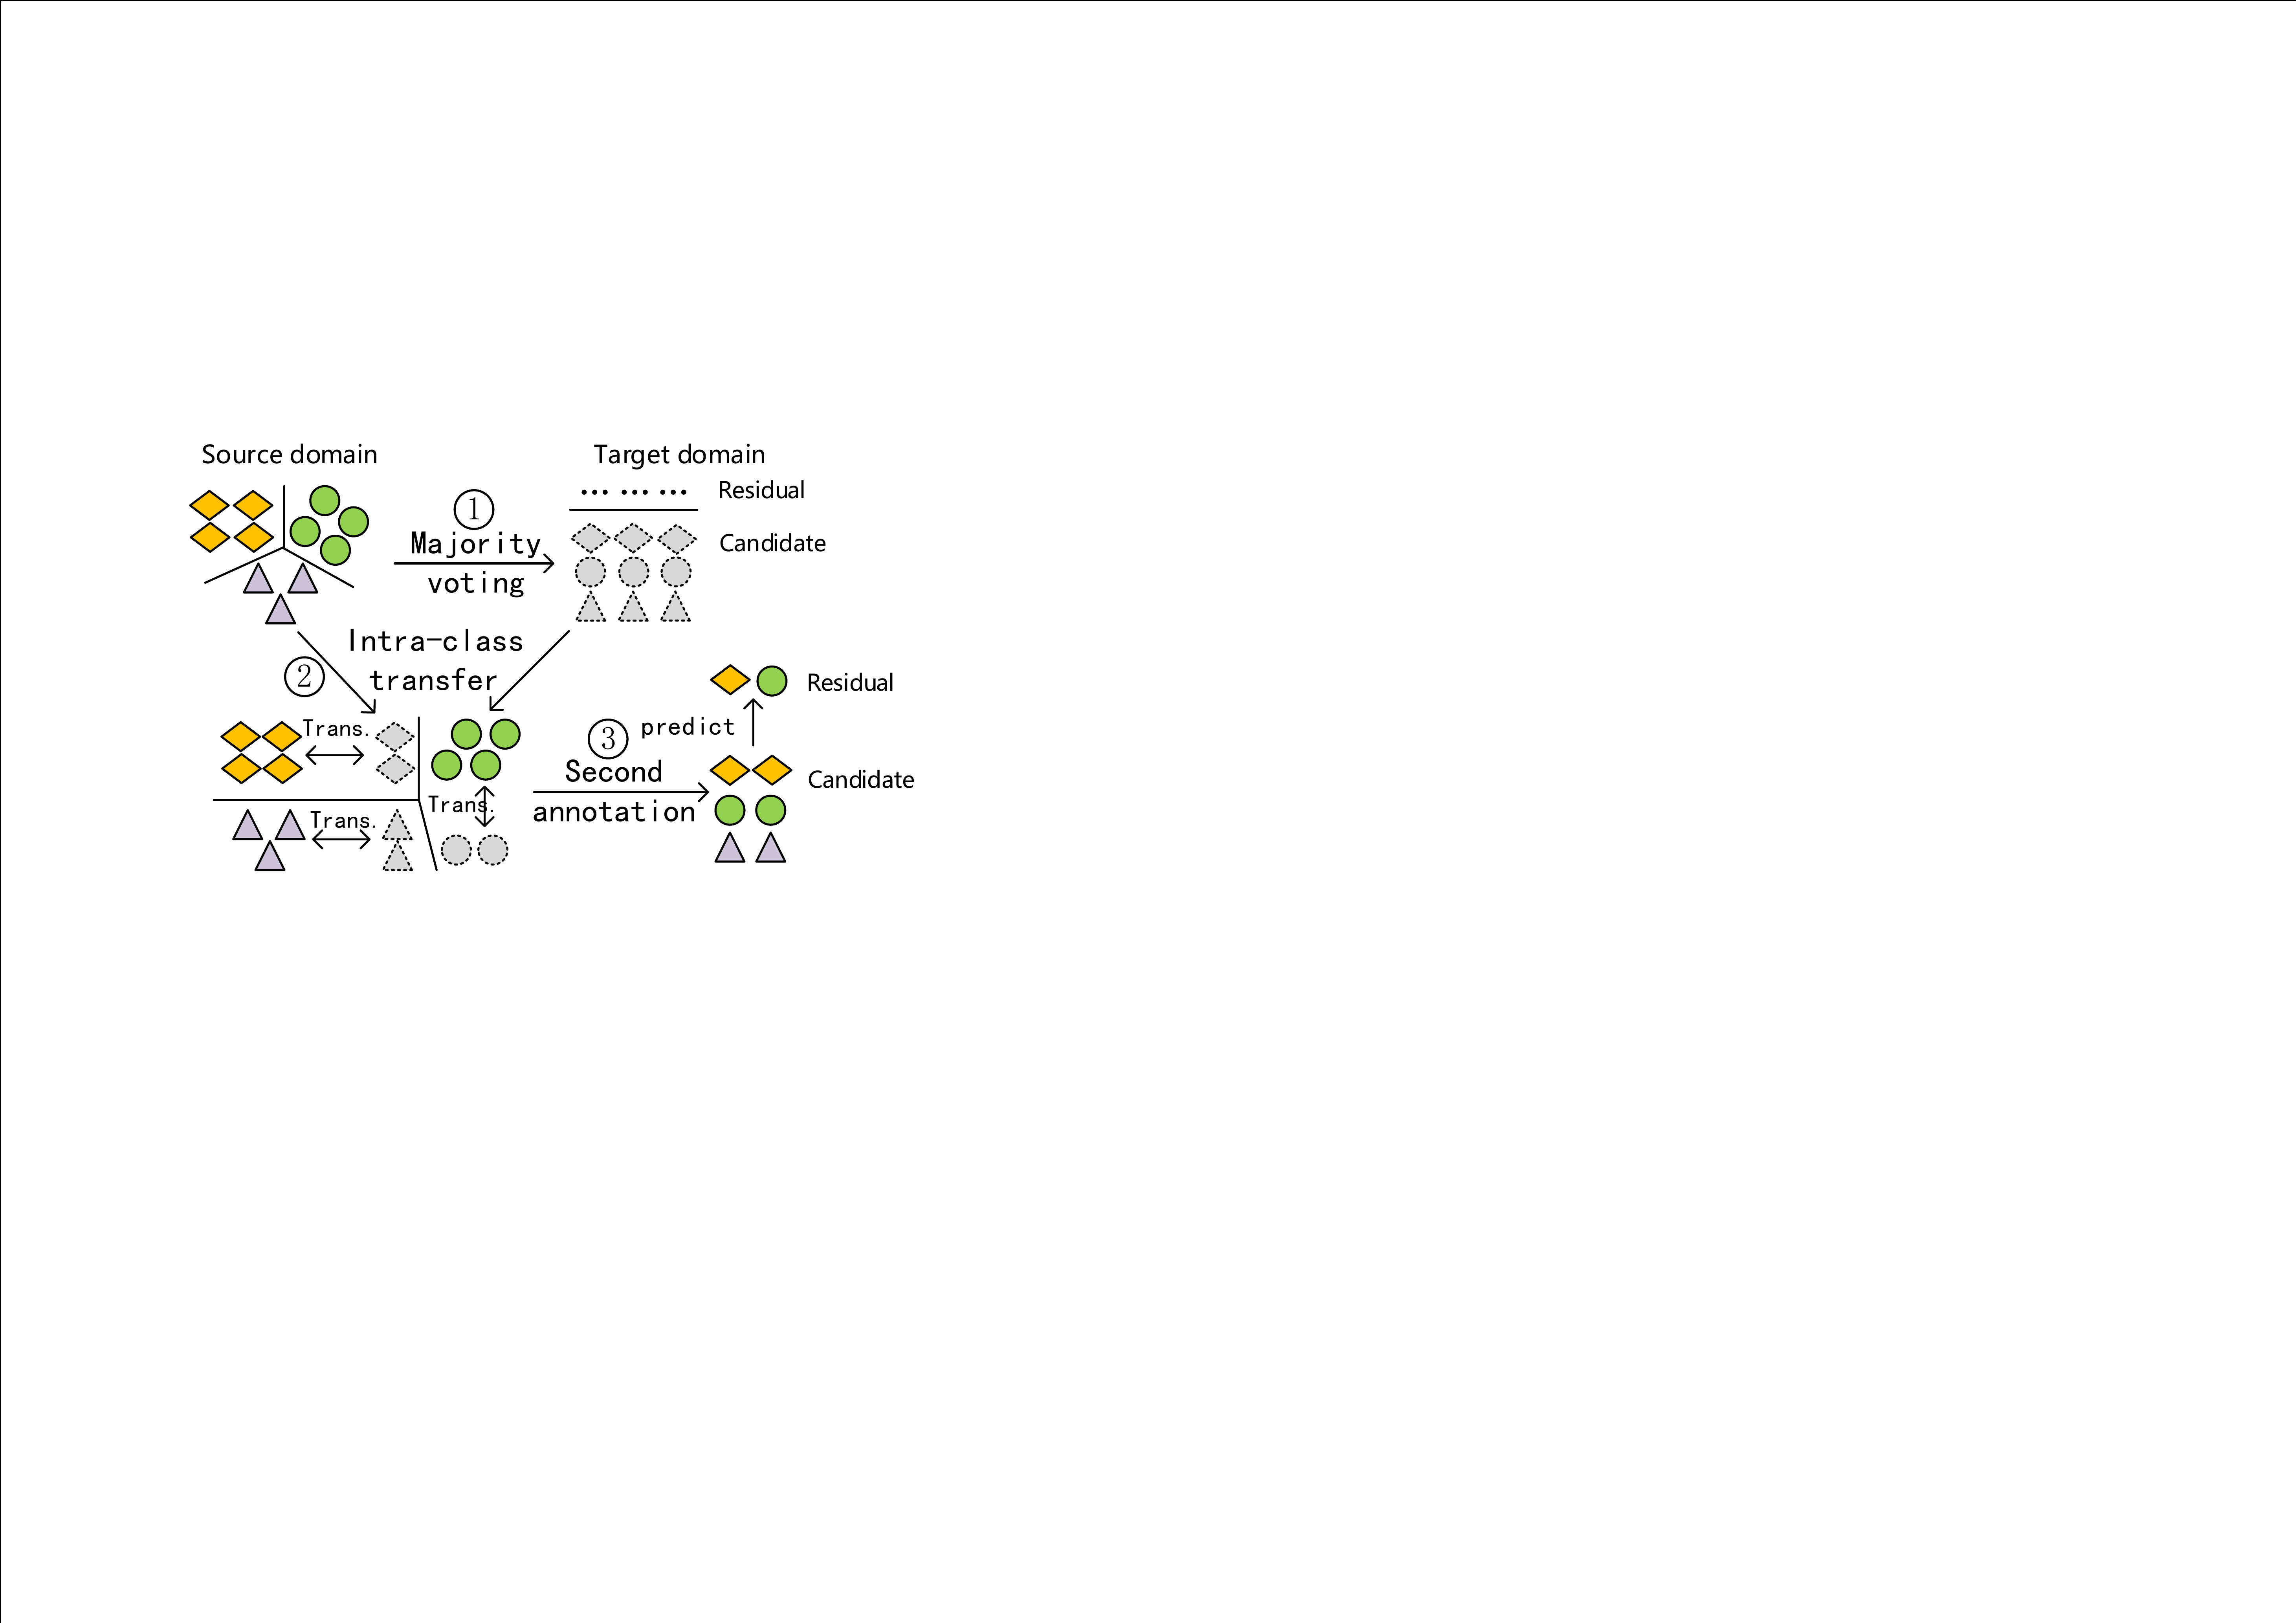
\includegraphics[scale=0.85]{./figures/fig-distribution-stl.pdf}
	\caption{STL方法的示意图}
	\label{fig-distribution-stl}
\end{figure}

为了实现\textit{类内迁移},我们需要计算每一类别的MMD距离。由于目标域没有标记,作者使用来自大多数投票结果中的伪标记。更加准确地说,用$c \in \{1, 2, \cdots, C\}$来表示类别标记,则类内迁移可以按如下方式计算:

\begin{equation}
\label{equ-stl-stra}
D(\mathcal{D}_{s},\mathcal{D}_{t})
=\sum_{c=1}^{C}\left \Vert \frac{1}{n^{(c)}_1} \sum_{\mathbf{x}_i \in \mathcal{D}^{(c)}_s} \phi(\mathbf{x}_i) - \frac{1}{n^{(c)}_2} \sum_{\mathbf{x}_j \in \mathcal{D}^{(c)}_t} \phi(\mathbf{x}_j) \right \Vert ^2_\mathcal{H}
\end{equation}

其中,$\mathcal{D}^{(c)}_s$和$\mathcal{D}^{(c)}_t$分别表示源域和目标域中属于类别$c$的样本。$n^{(c)}_1=|\mathcal{D}^{(c)}_s|$,且$n^{(c)}_2=|\mathcal{D}_t|$。

接下来的步骤请参照STL方法原文进行理解。

STL方法在大量行为识别数据中进行了跨位置行为识别的实验。实验结果表明,该方法可以很好地实现跨领域的行为识别任务,取得了当前最好的效果。

\subsection{联合分布自适应}

\subsubsection{基本思路}

联合分布自适应方法(Joint Distribution Adaptation)的目标是减小源域和目标域的联合概率分布的距离,从而完成迁移学习。从形式上来说,联合分布自适应方法是用$P(\mathbf{x}_s)$和$P(\mathbf{x}_t)$之间的距离、以及$P(y_s|\mathbf{x}_s)$和$P(y_t|\mathbf{x}_t)$之间的距离来近似两个领域之间的差异。即:

\begin{equation}
\label{eq-joint-general}
DISTANCE(\mathcal{D}_s,\mathcal{D}_t) \approx ||P(\mathbf{x}_s) - P(\mathbf{x}_t)|| + ||P(y_s|\mathbf{x}_s) - P(y_t|\mathbf{x}_t)||
\end{equation}

联合分布自适应对应于图~\ref{fig-distribution}中由图~\ref{fig-distribution-source}迁移到图~\ref{fig-distribution-target1}的情形、以及图~\ref{fig-distribution-source}迁移到图~\ref{fig-distribution-target2}的情形。

\subsubsection{核心方法}

联合分布适配的JDA方法~\cite{long2013transfer}首次发表于2013年的ICCV(计算机视觉领域顶会,与CVPR类似),它的作者是当时清华大学的博士生(现为清华大学助理教授)龙明盛。

假设是最基本的出发点。那么JDA这个方法的假设是什么呢?就是假设两点:1)源域和目标域边缘分布不同,2)源域和目标域条件分布不同。既然有了目标,同时适配两个分布不就可以了吗?于是作者很自然地提出了联合分布适配方法:适配联合概率。

不过这里我感觉有一些争议:边缘分布和条件分布不同,与联合分布不同并不等价。所以这里的“联合”二字实在是会引起歧义。我的理解是,同时适配两个分布,也可以叫联合,而不是概率上的“联合”。尽管作者在文章里第一个公式就写的是适配联合概率,但是这里感觉是有一些问题的。我们抛开它这个有歧义的,把“联合”理解成同时适配两个分布。

那么,JDA方法的目标就是,寻找一个变换$\mathbf{A}$,使得经过变换后的$P(\mathbf{A}^\top \mathbf{x}_s)$和$P(\mathbf{A}^\top \mathbf{x}_t)$的距离能够尽可能地接近,同时,$P(y_s|\mathbf{A}^\top \mathbf{x}_s)$和$P(y_t|\mathbf{A}^\top \mathbf{x}_t)$的距离也要小。很自然地,这个方法也就分成了两个步骤。

\textit{边缘分布适配}

首先来适配边缘分布,也就是$P(\mathbf{A}^\top \mathbf{x}_s)$和$P(\mathbf{A}^\top \mathbf{x}_t)$的距离能够尽可能地接近。其实这个操作就是迁移成分分析(TCA)。我们仍然使用MMD距离来最小化源域和目标域的最大均值差异。MMD距离是

\begin{equation}
	\left \Vert \frac{1}{n} \sum_{i=1}^{n} \mathbf{A}^\top \mathbf{x}_{i} - \frac{1}{m} \sum_{j=1}^{m} \mathbf{A}^\top \mathbf{x}_{j} \right \Vert ^2_\mathcal{H}
\end{equation}

这个式子实在不好求解。我们引入核方法,化简这个式子,它就变成了

\begin{equation}
	D(\mathcal{D}_s,\mathcal{D}_t)=tr(\mathbf{A}^\top \mathbf{X} \mathbf{M}_0 \mathbf{X}^\top \mathbf{A})
\end{equation}

其中$\mathbf{A}$就是变换矩阵,我们把它加黑加粗,$\mathbf{X}$是源域和目标域合并起来的数据。$\mathbf{M}_0$是一个MMD矩阵:

\begin{equation}
	(\mathbf{M}_0)_{ij}=\begin{cases} \frac{1}{n^2}, & \mathbf{x}_i,\mathbf{x}_j \in \mathcal{D}_s\\ \frac{1}{m^2}, & \mathbf{x}_i,\mathbf{x}_j \in \mathcal{D}_t\\ -\frac{1}{mn}, & \text{otherwise} \end{cases}
\end{equation}

$n,m$分别是源域和目标域样本的个数。

到此为止没有什么创新点,因为这就是一个TCA。

\textit{条件分布适配}

这是我们要做的第二个目标,适配源域和目标域的条件概率分布。也就是说,还是要找一个变换$\mathbf{A}$,使得$P(y_s|\mathbf{A}^\top \mathbf{x}_s)$和$P(y_t|\mathbf{A}^\top \mathbf{x}_t)$的距离也要小。那么简单了,我们再用一遍MMD啊。可是问题来了:我们的目标域里,没有$y_t$,没法求目标域的条件分布!

这条路看来是走不通了。也就是说,直接建模$P(y_t|\mathbf{x}_t)$不行。那么,能不能有别的办法可以逼近这个条件概率?我们可以换个角度,利用类条件概率$P(\mathbf{x}_t|y_t)$。根据贝叶斯公式$P(y_t|\mathbf{x}_t)=p(y_t)p(\mathbf{x}_t|y_t)$,我们如果忽略$P(\mathbf{x}_t)$,那么岂不是就可以用$P(\mathbf{x}_t|y_t)$来近似$P(y_t|\mathbf{x}_t)$?

而这样的近似也不是空穴来风。在统计学上,有一个概念叫做\textit{充分统计量},它是什么意思呢?大概意思就是说,如果样本里有太多的东西未知,样本足够好,我们就能够从中选择一些统计量,近似地代替我们要估计的分布。好了,我们为近似找到了理论依据。

实际怎么做呢?我们依然没有$y_t$。采用的方法是,用$(\mathbf{x}_s,y_s)$来训练一个简单的分类器(比如knn、逻辑斯特回归),到$\mathbf{x}_t$上直接进行预测。总能够得到一些伪标签$\hat{y}_t$。我们根据伪标签来计算,这个问题就可解了。

类与类之间的MMD距离表示为

\begin{equation}
	\sum_{c=1}^{C}\left \Vert \frac{1}{n_c} \sum_{\mathbf{x}_{i} \in \mathcal{D}^{(c)}_s} \mathbf{A}^\top \mathbf{x}_{i} - \frac{1}{m_c} \sum_{\mathbf{x}_{i} \in \mathcal{D}^{(c)}_t} \mathbf{A}^\top \mathbf{x}_{i} \right \Vert ^2_\mathcal{H}
\end{equation}

其中,$n_c,m_c$分别标识源域和目标域中来自第$c$类的样本个数。同样地我们用核方法,得到了下面的式子

\begin{equation}
	\sum_{c=1}^{C}tr(\mathbf{A}^\top \mathbf{X} \mathbf{M}_c \mathbf{X}^\top \mathbf{A})
\end{equation}

其中$\mathbf{M}_c$为

\begin{equation}
	(\mathbf{M}_c)_{ij}=\begin{cases} \frac{1}{n^2_c}, & \mathbf{x}_i,\mathbf{x}_j \in \mathcal{D}^{(c)}_s\\ \frac{1}{m^2_c}, & \mathbf{x}_i,\mathbf{x}_j \in \mathcal{D}^{(c)}_t\\ -\frac{1}{m_c n_c}, & \begin{cases} \mathbf{x}_i \in \mathcal{D}^{(c)}_s ,\mathbf{x}_j \in \mathcal{D}^{(c)}_t \\ \mathbf{x}_i \in \mathcal{D}^{(c)}_t ,\mathbf{x}_j \in \mathcal{D}^{(c)}_s \end{cases}\\ 0, & \text{otherwise}\end{cases}
\end{equation}

现在我们把两个距离结合起来,得到了一个总的优化目标:

\begin{equation}
	\min \sum_{c=0}^{C}tr(\mathbf{A}^\top \mathbf{X} \mathbf{M}_c \mathbf{X}^\top \mathbf{A}) + \lambda \Vert \mathbf{A} \Vert ^2_F
\end{equation}

看到没,通过$c=0 \cdots C$就把两个距离统一起来了!其中的$\lambda \Vert \mathbf{A} \Vert ^2_F$是正则项,使得模型是\textit{良好定义}(Well-defined)的。

我们还缺一个限制条件,不然这个问题无法解。限制条件是什么呢?和TCA一样,变换前后数据的方差要维持不变。怎么求数据的方差呢,还和TCA一样:$\mathbf{A}^\top \mathbf{X} \mathbf{H} \mathbf{X}^\top \mathbf{A} = \mathbf{I}$,其中的$\mathbf{H}$也是中心矩阵,$\mathbf{I}$是单位矩阵。也就是说,我们又添加了一个优化目标是要$\max \mathbf{A}^\top \mathbf{X} \mathbf{H} \mathbf{X}^\top \mathbf{A}$(这一个步骤等价于PCA了)。和原来的优化目标合并,优化目标统一为:

\begin{equation}
	\min \frac{\sum_{c=0}^{C}tr(\mathbf{A}^\top \mathbf{X} \mathbf{M}_c \mathbf{X}^\top \mathbf{A}) + \lambda \Vert \mathbf{A}\Vert^2_F}{ \mathbf{A}^\top \mathbf{X} \mathbf{H} \mathbf{X}^\top \mathbf{A}}
\end{equation}

这个式子实在不好求解。但是,有个东西叫做Rayleigh quotient~\footnote{\url{https://www.wikiwand.com/en/Rayleigh_quotient}},上面两个一样的这种形式。因为$\mathbf{A}$是可以进行拉伸而不改变最终结果的,而如果下面为0的话,整个式子就求不出来值了。所以,我们直接就可以让下面不变,只求上面。所以我们最终的优化问题形式搞成了

\begin{equation}
	\min \quad \sum_{c=0}^{C}tr(\mathbf{A}^\top \mathbf{X} \mathbf{M}_c \mathbf{X}^\top \mathbf{A}) + \lambda \Vert \mathbf{A} \Vert ^2_F \quad \text{s.t.} \quad \mathbf{A}^\top \mathbf{X} \mathbf{H} \mathbf{X}^\top \mathbf{A} = \mathbf{I}
\end{equation}

怎么解?太简单了,可以用拉格朗日法。最后变成了

\begin{equation}
	\left(\mathbf{X} \sum_{c=0}^{C} \mathbf{M}_c \mathbf{X}^\top + \lambda \mathbf{I}\right) \mathbf{A} =\mathbf{X} \mathbf{H} \mathbf{X}^\top \mathbf{A} \Phi 
\end{equation}

其中的$\Phi$是拉格朗日乘子。别看这个东西复杂,又有要求解的$\mathbf{A}$,又有一个新加入的$\Phi$ 。但是它在Matlab里是可以直接解的(用$\mathrm{eigs}$函数即可)。这样我们就得到了变换$\mathbf{A}$,问题解决了。

可是伪标签终究是伪标签啊,肯定精度不高,怎么办?有个东西叫做\textit{迭代},一次不行,我们再做一次。后一次做的时候,我们用上一轮得到的标签来作伪标签。这样的目的是得到越来越好的伪标签,而参与迁移的数据是不会变的。这样往返多次,结果就自然而然好了。

JDA方法是十分经典的迁移学习方法。后续的相关工作通过在JDA的基础上加入额外的损失项,使得迁移学习的效果得到了很大提升。我们在这里简要介绍一些基于JDA的相关工作。

\begin{itemize}
	\item ARTL~(Adaptation Regularization)~\cite{long2014adaptation}: 将JDA嵌入一个结构风险最小化框架中,用表示定理直接学习分类器
	\item VDA~\cite{tahmoresnezhad2016visual}: 在JDA的优化目标中加入了类内距和类间距的计算
	\item \cite{hsiao2016learning}: 在JDA的基础上加入结构不变性控制
	\item \cite{hou2015unsupervised}: 在JDA的基础上加入目标域的选择
	\item JGSA~(Joint Geometrical and Statistical Alignment)~\cite{zhang2017joint}: 在JDA的基础上加入类内距、类间距、标签持久化
	\item JAN~(Joint Adaptation Network)~\cite{long2017deep}: 提出了联合分布度量JMMD,在深度网络中进行联合分布的优化
\end{itemize}

\subsection{动态分布自适应}

\textbf{平衡分布自适应BDA}

在最近的研究中,来自中科院计算所的Wang等人~\cite{wang2017balanced}注意到了JDA的不足:\textit{边缘分布自适应和条件分布自适应并不是同等重要}。回到图~\ref{fig-distribution}表示的两种分布的问题上来。显然,当目标域是图~\ref{fig-distribution-target1}所示的情况时,边缘分布应该被优先考虑;而当目标域是图~\ref{fig-distribution-target2}所示的情况时,条件分布应该被优先考虑。JDA以及后来的扩展工作均忽视了这一问题。

作者提出了BDA方法(Balanced Distribution Adaptation)来解决这一问题。该方法能够根据特定的数据领域,自适应地调整分布适配过程中边缘分布和条件分布的重要性。准确而言,BDA通过采用一种\textit{平衡因子}$\mu$来动态调整两个分布之间的距离
\begin{equation}
\label{equ-mummd}
\begin{split}
DISTANCE(\mathcal{D}_s,\mathcal{D}_t) \approx  (1 &- \mu)DISTANCE(P(\mathbf{x}_s),P(\mathbf{x}_t))\\
&+ \mu DISTANCE(P(y_s|\mathbf{x}_s),P(y_t|\mathbf{x}_t))
\end{split}
\end{equation}
其中$\mu \in [0,1]$表示平衡因子。当$\mu \rightarrow 0$,这表示源域和目标域数据本身存在较大的差异性,因此,边缘分布适配更重要;当$\mu \rightarrow 1$时,这表示源域和目标域数据集有较高的相似性,因此,条件概率分布适配更加重要。综合上面的分析可知,平衡因子可以根据实际数据分布的情况,动态地调节每个分布的重要性,并取得良好的分布适配效果。

其中的平衡因子$\mu$可以通过分别计算两个领域数据的整体和局部的$\mathcal{A}$-distance近似给出。特别地,当$\mu = 0$时,方法退化为TCA;当$\mu = 0.5$时,方法退化为JDA。

我们采用BDA文章中的图来具体地展示出$\mu$的作用。图~\ref{fig-distribution-bda}的结果清晰地显示出,平衡因子可以取得比JDA、TCA更小的MMD距离、更高的精度。

%\begin{figure}[htbp]
%	\centering
%	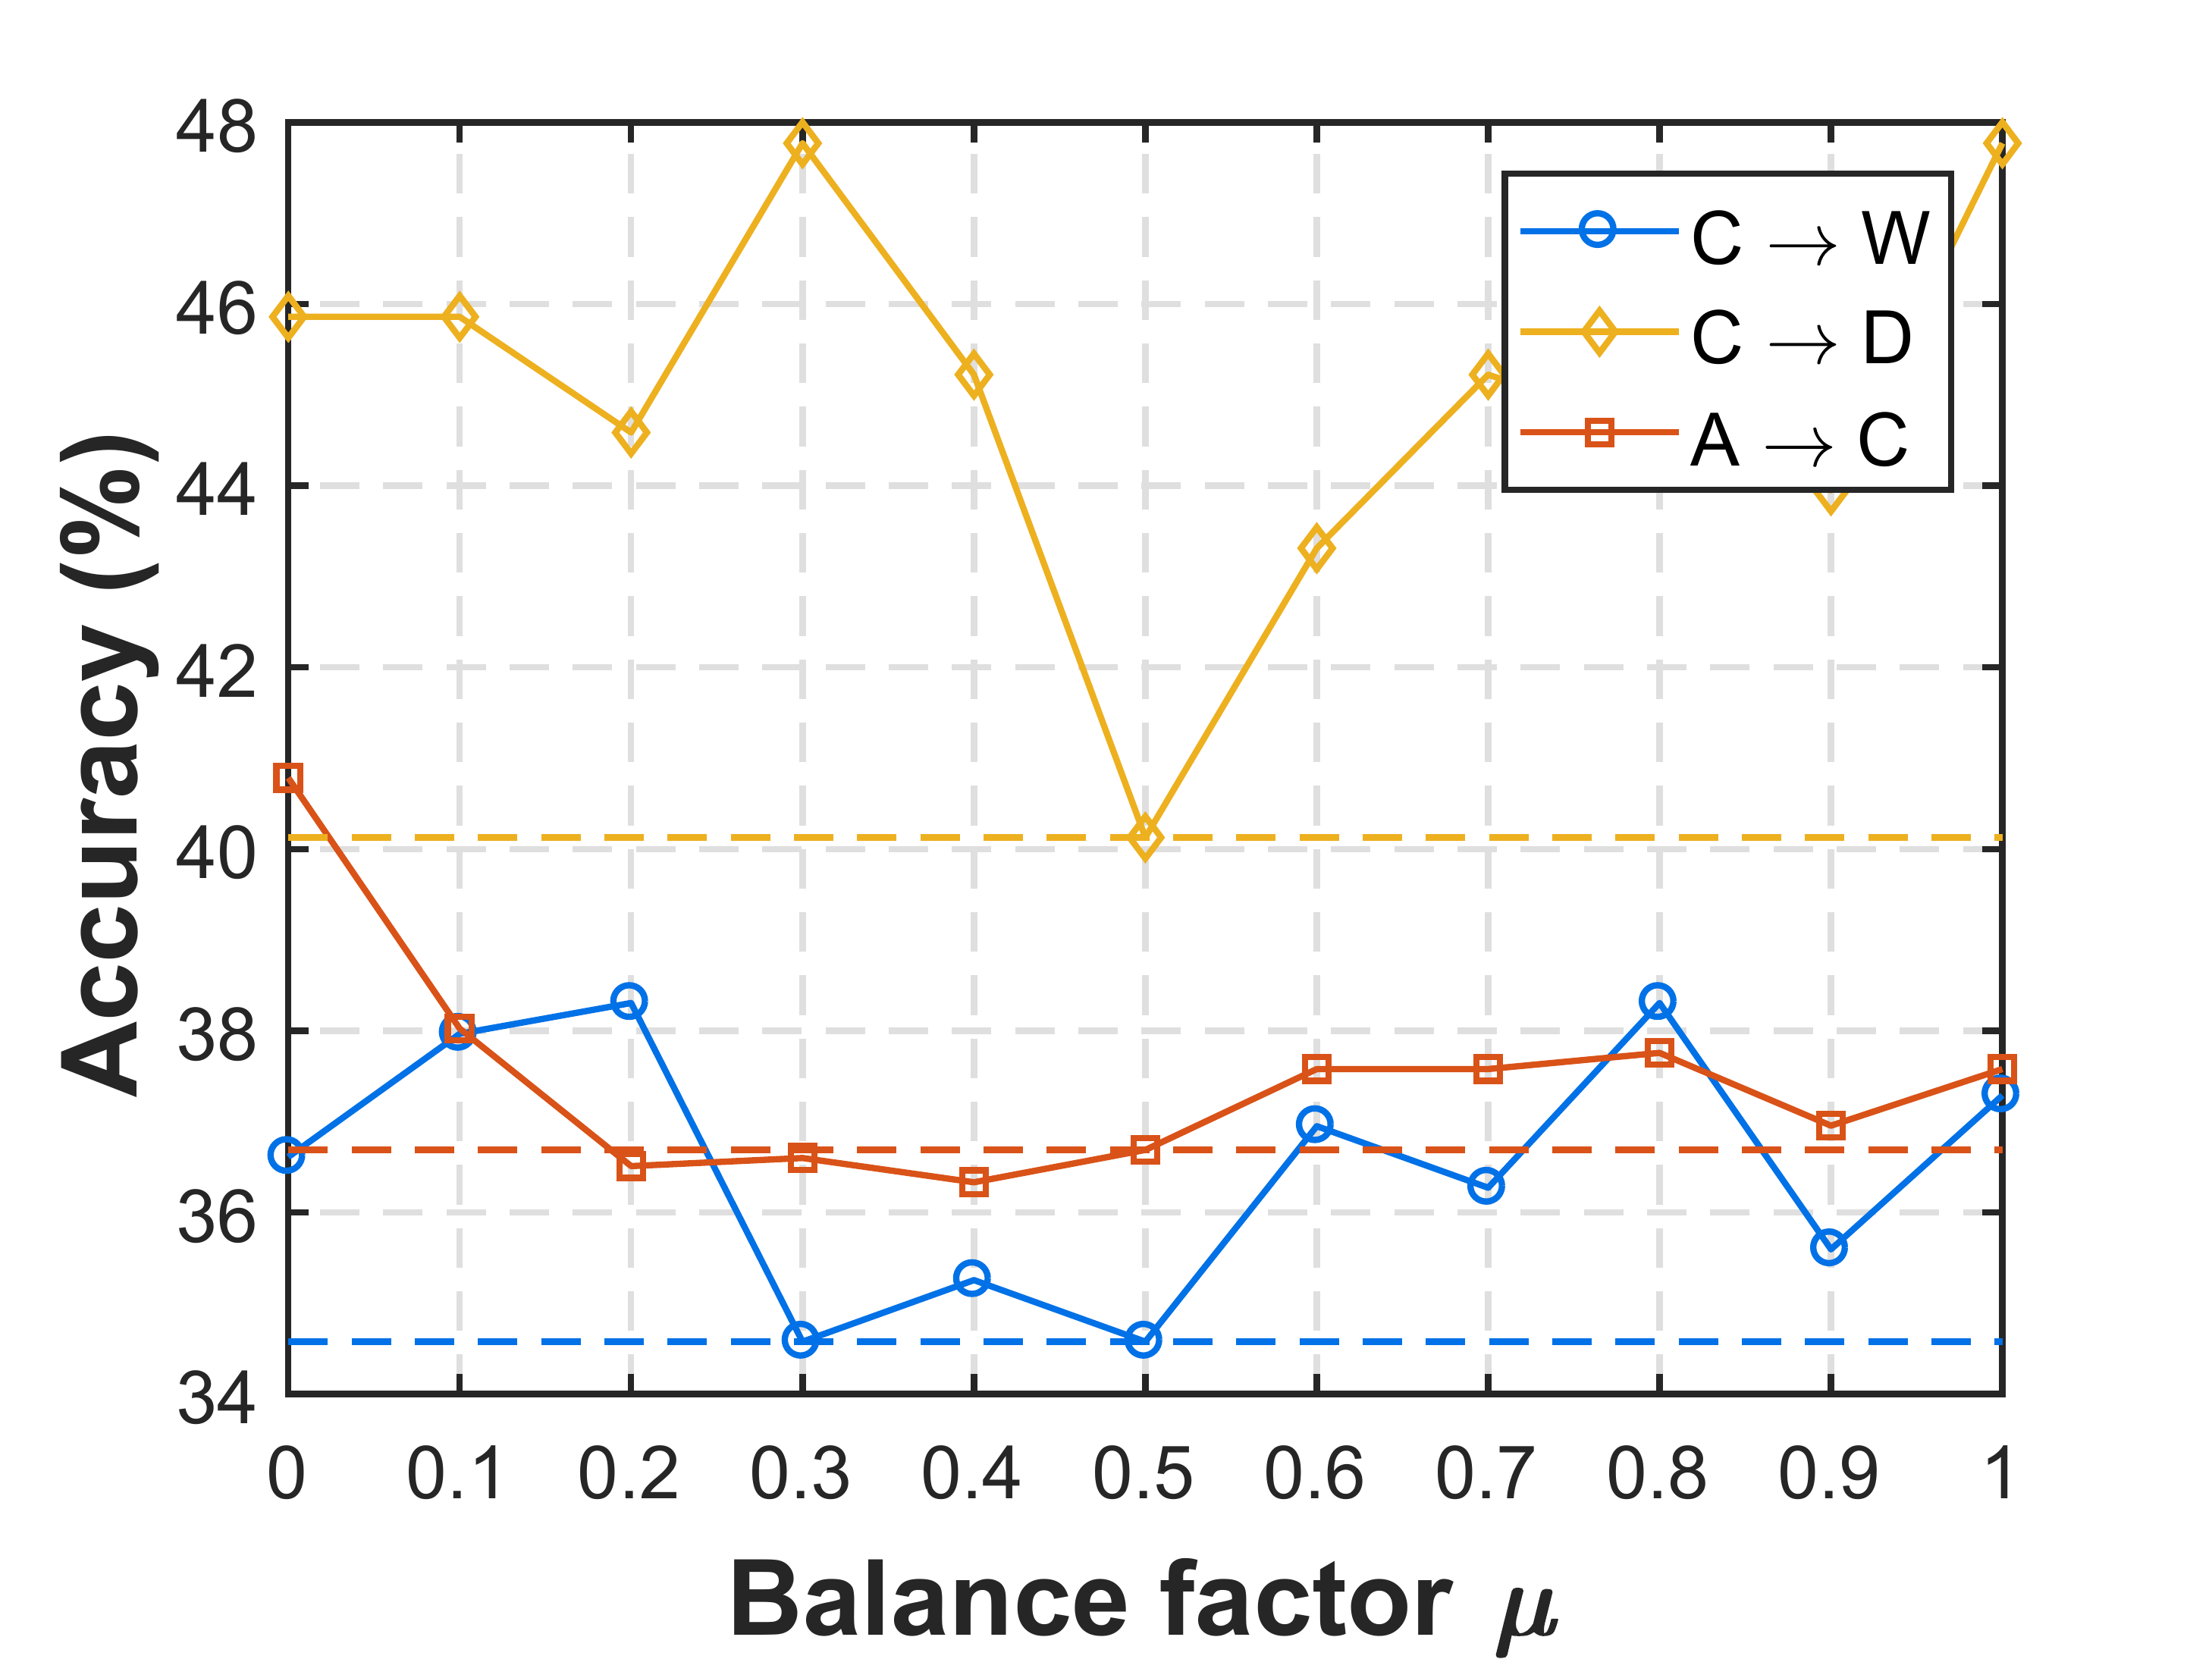
\includegraphics[scale=0.6]{./figures/fig-distribution-mu.pdf}
%	\caption{平衡因子$\mu$在分布自适应中的作用}
%	\label{fig-distribution-mu}
%\end{figure}

\begin{figure*}[h]
	\centering
	\subfigure[不同方法的MMD距离比较]{
		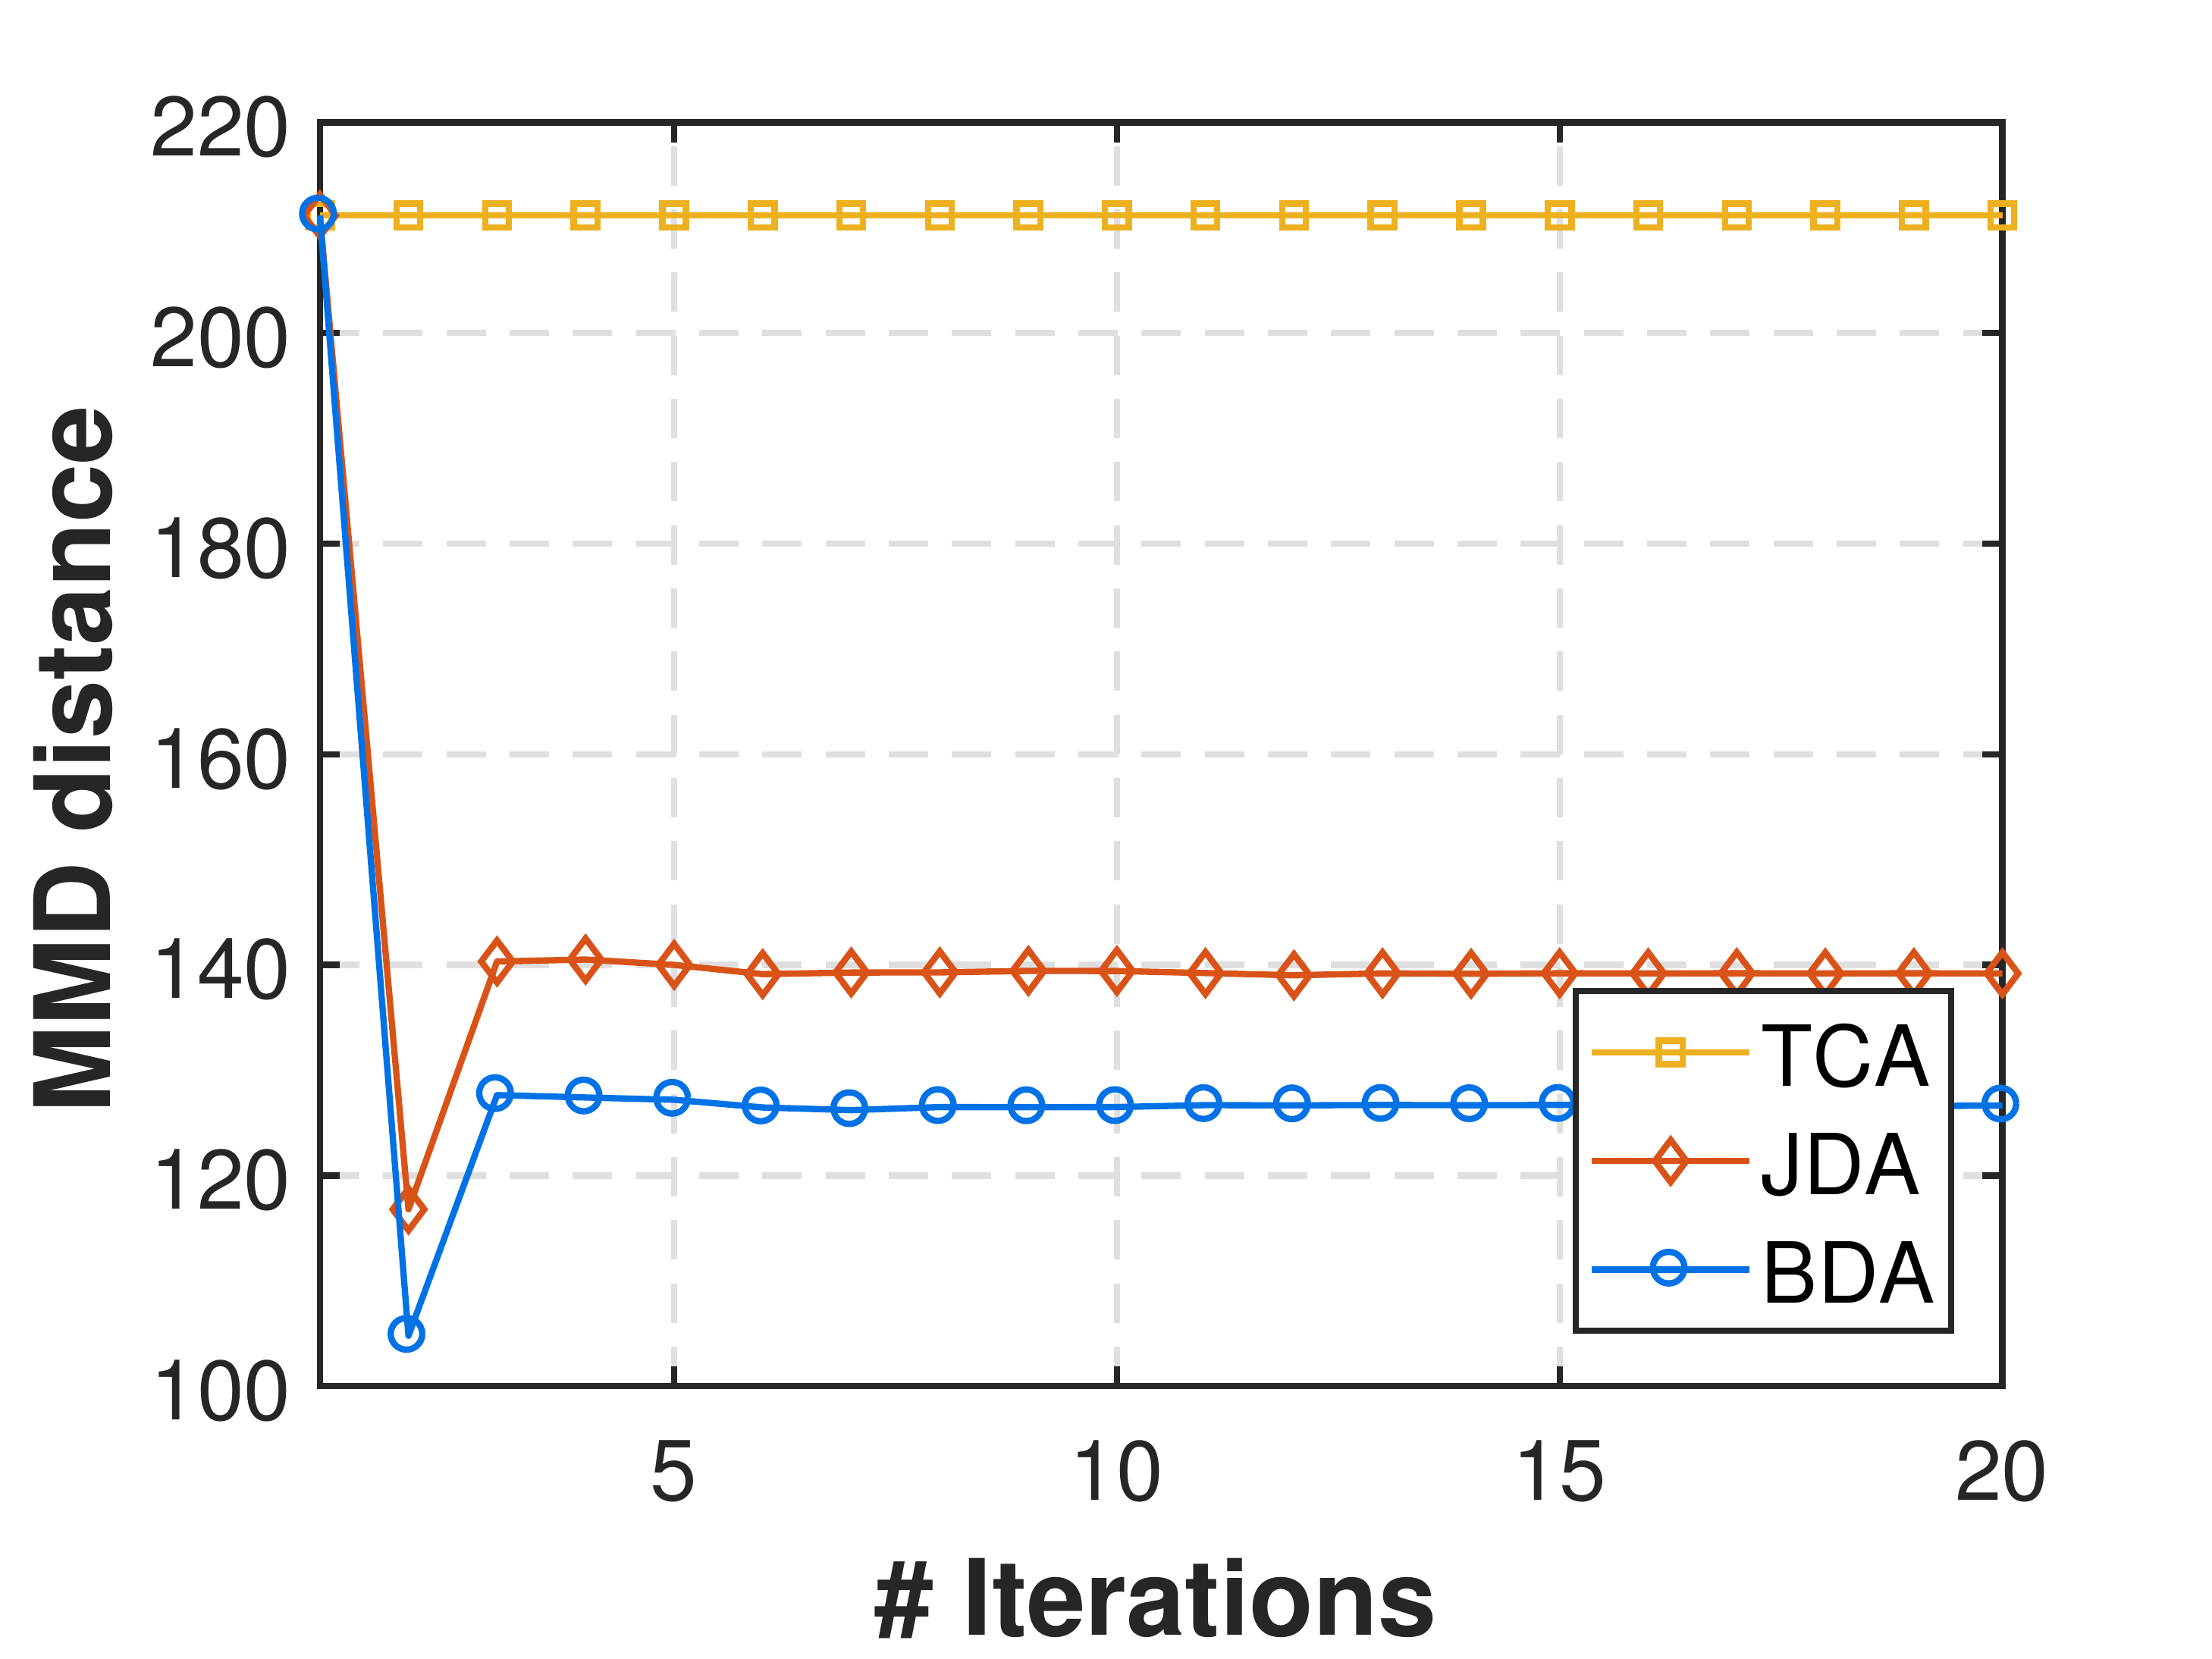
\includegraphics[scale=0.45]{./figures/fig-distribution-bdammd.pdf}
		\label{fig-distribution-mmd}}

	\subfigure[BDA方法中平衡因子$\mu$的作用]{
		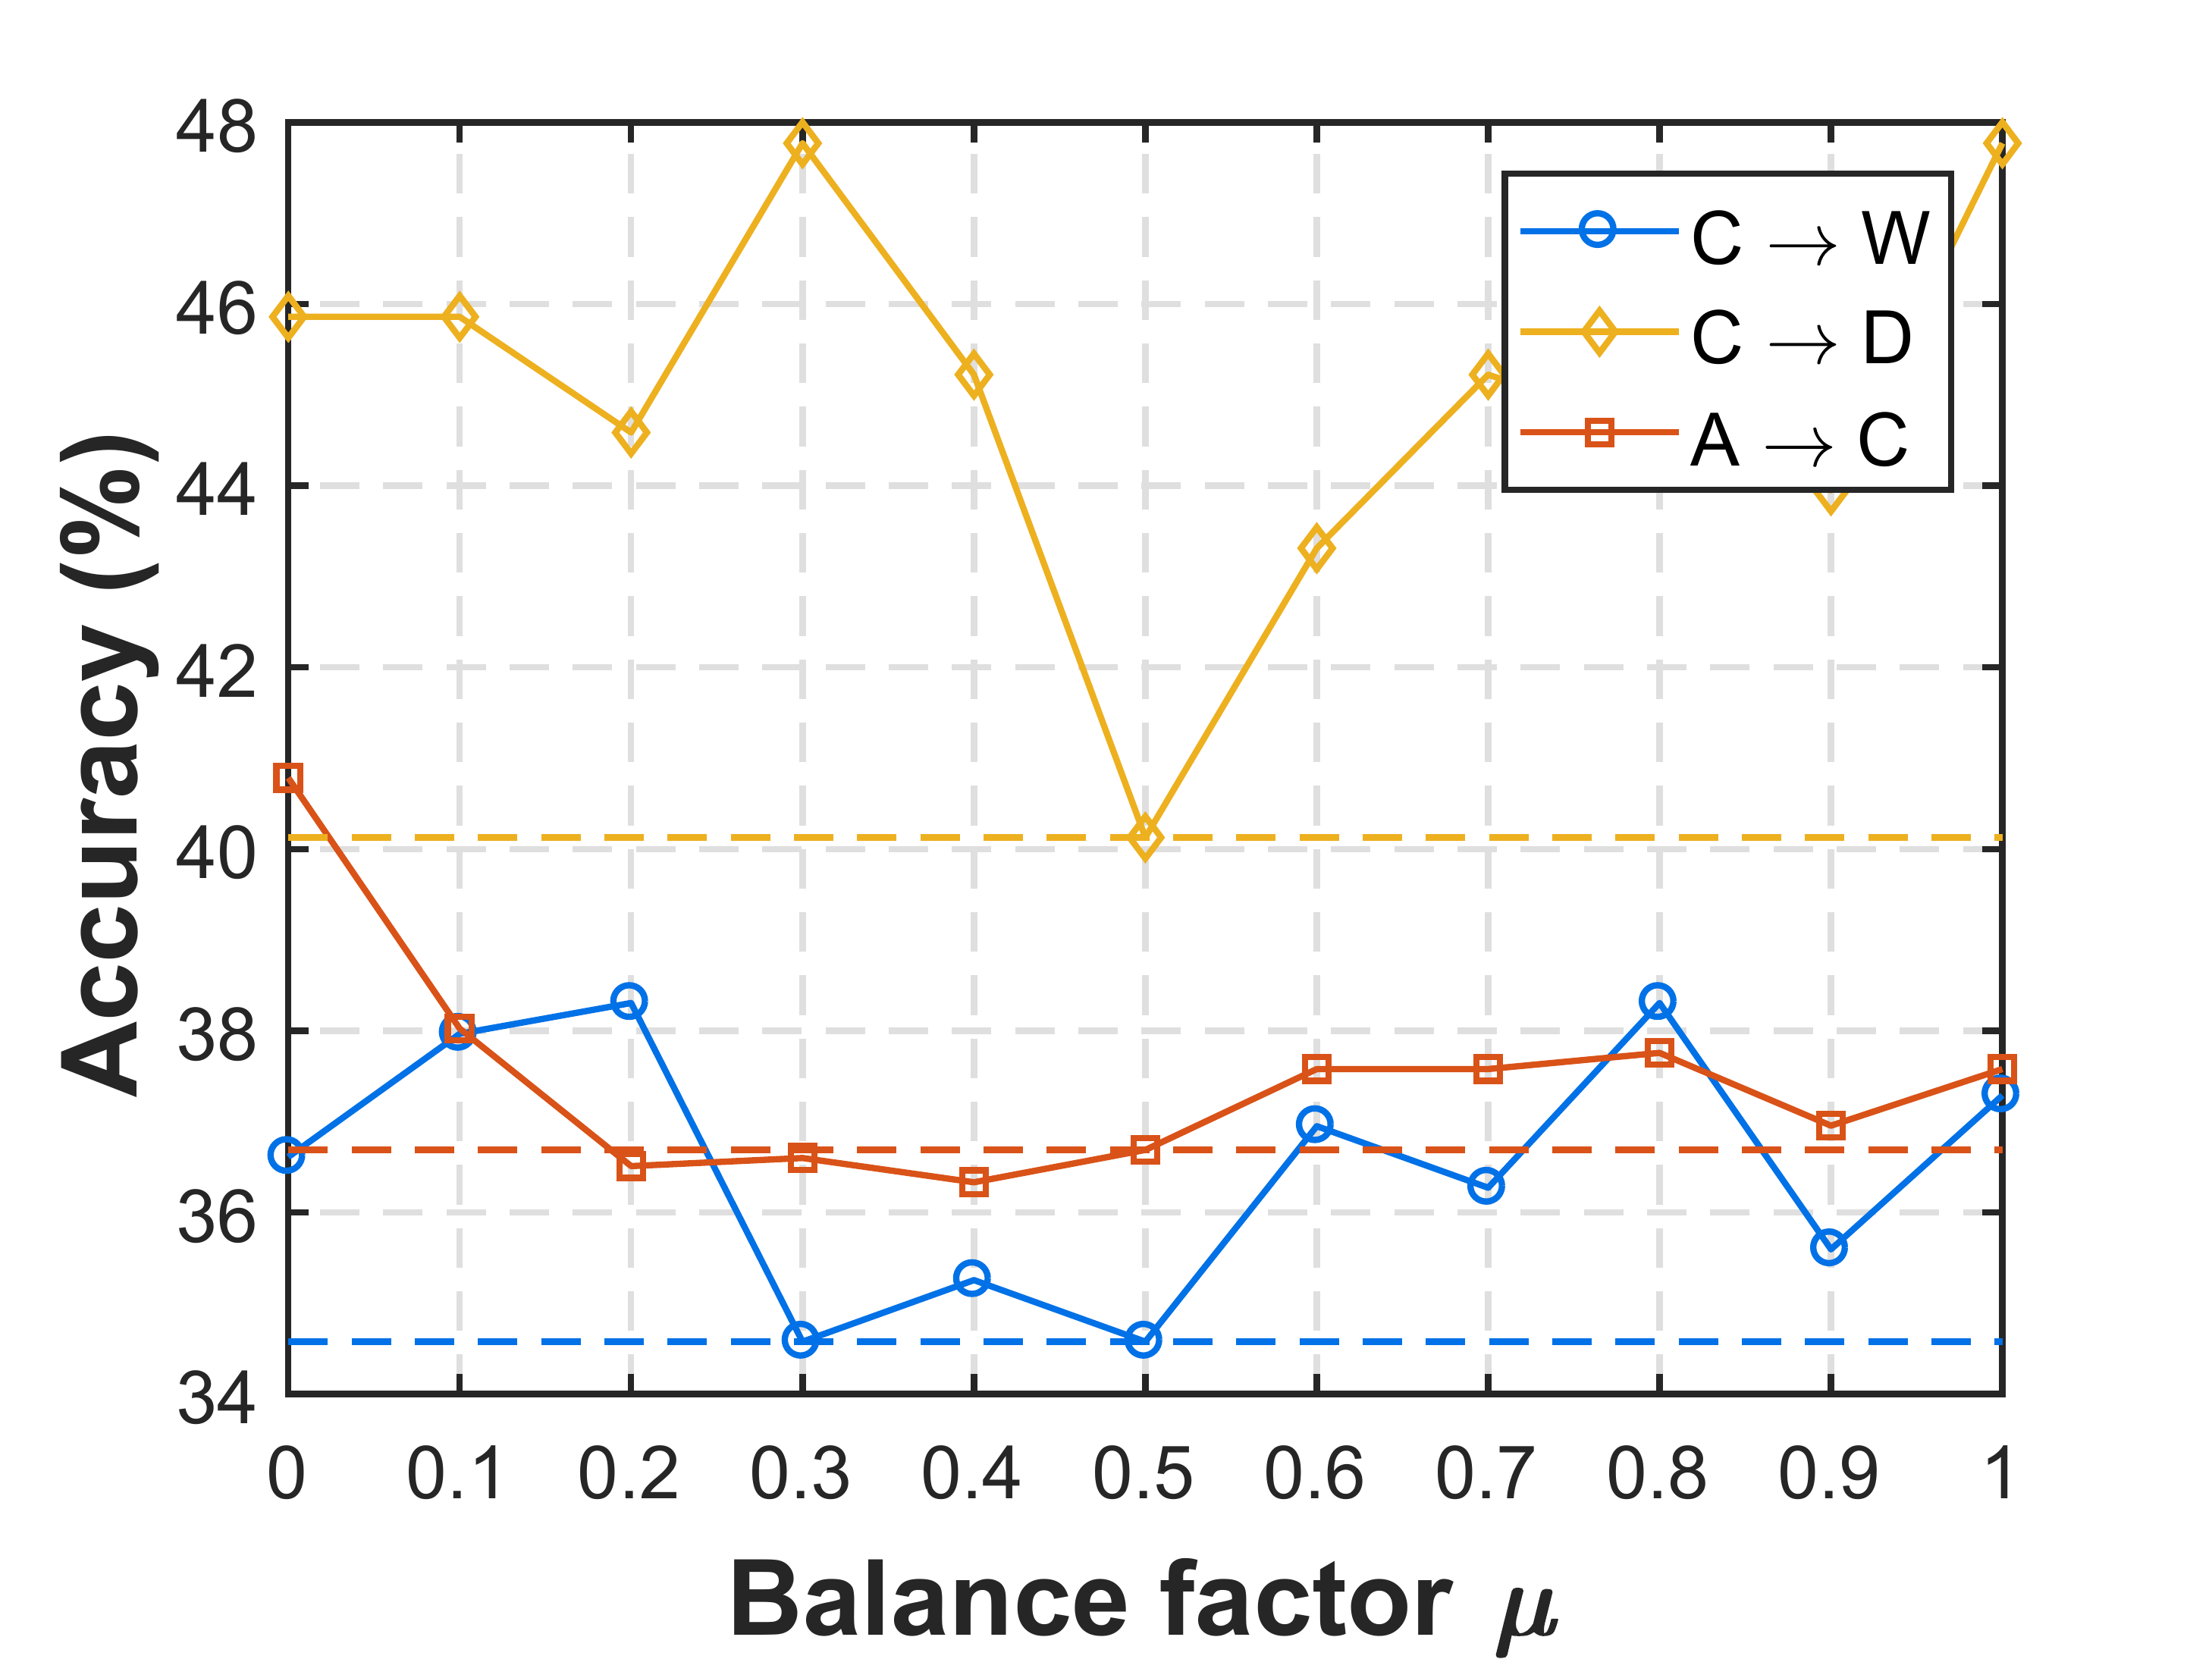
\includegraphics[scale=0.45]{./figures/fig-distribution-mu.pdf}
		\label{fig-distribution-mu}}
	\caption{BDA方法的效果}
	\label{fig-distribution-bda}
\end{figure*}

\textbf{动态分布自适应}

BDA方法是首次给出边缘分布和条件分布的定量估计。然而,其并未解决平衡因子$\mu$的精确计算问题。最近,作者扩展了BDA方法,提出了一个更具普适性的动态迁移框架DDA(Dynamic Distribution Adaptation)~\cite{wang2019transfer}来解决$\mu$值的精确估计问题。

注意到,可以简单地将$\mu$视为一个迁移过程中的参数,通过交叉验证 (cross-validation)来确定其最优的取值$\mu_{opt}$。然而,在本章的无监督迁移学习问题定义中,目标域完全没有标记,故此方式不可行。有另外两种非直接的方式可以对$\mu$值进行估计:随机猜测和最大最小平均法。随机猜测从神经网络随机调参中得到启发,指的是任意从$[0,1]$区间内选择一个$\mu$的值,然后进行动态迁移,其并不算是一种技术严密型的方案。如果重复此过程$t$次,记第$t$次的迁移学习结果为$r_t$,则随机猜测法最终的迁移结果为$r_{rand} = \frac{1}{t} \sum_{i=1}^{t} r_t$。最大最小平均法与随机猜测法相似,可以在$[0,1]$区间内从0开始取$\mu$的值,每次增加0.1,得到一个集合$[0,0.1,\cdots,0.9,1.0]$,然后,与随机猜测法相似,也可以得到其最终迁移结果$r_{maxmin}=\frac{1}{11} \sum_{i=1}^{11} r_i$。

然而,尽管上述两种估计方案有一定的可行性,它们均需要大量的重复计算,给普适计算设备带来了严峻的挑战。另外,上述结果并不具有可解释性,其正确性也无法得到保证。

作者提出的动态迁移方法是首次对$\mu$值进行精确的定量估计方法。该方法利用领域的整体和局部性质来定量计算$\mu$(计算出的值用$\hat{\mu}$来表示)。采用$\mathcal{A}-distance$~\cite{ben2007analysis}作为基本的度量方式。$\mathcal{A}-distance$被定义为建立一个二分类器进行两个不同领域的分类得出的误差。从形式化来看,定义$\epsilon(h)$作为线性分类器$h$区分两个领域$\Omega_s$和$\Omega_t$的误差。则,$\mathcal{A}-distance$可以被定义为:
\begin{equation}
d_A(\Omega_s,\Omega_t) = 2(1 - 2 \epsilon(h)).
\end{equation}

直接根据上式计算边缘分布的$\mathcal{A}-distance$,将其用$d_M$来表示。对于条件分布之间的$\mathcal{A}-distance$,用$d_c$来表示对应于类别$c$的条件分布距离。它可以由式$d_c = d_A(\Omega^{(c)}_s,\Omega^{(c)}_t)$进行计算,其中$\Omega^{(c)}_s$和$\Omega^{(c)}_t$分别表示来自源域和目标域的第$c$个类的样本。最终,$\mu$可以由下式进行计算:
\begin{equation}
\label{eq-meda-mu}
\hat{\mu} = 1 - \frac{d_M}{d_M + \sum_{c=1}^{C} d_c}.
\end{equation}

由于特征的动态和渐近变化性,此估计需要在每一轮迭代中给出。值得注意的是,这是\textbf{首次}给出边缘分布和条件分布的定量估计,对于迁移学习研究具有很大的意义。

具体而言,作者将机器学习问题规约成一个统计机器学习问题,可以用统计机器学习中的结构风险最小化的原则(Structural Risk Minimization, SRM)~\cite{belkin2006manifold,vapnik1998statistical}进行表示学习。在SRM中,分类器$f$可以被表示为:
\begin{equation}
\label{eq-meda-srm}
f = \mathop{\arg\min}_{f \in \mathcal{H}_{K}, (\mathbf{x},y) \sim \Omega_l} J(f(\mathbf{x}),y) + R(f),
\end{equation}
其中第一项表示$f$在有标记数据上的损失,第二项为正则项,$\mathcal{H}_{K}$表示核函数$K(\cdot,\cdot)$构造的希尔伯特空间 (Hilbert space)。符号$\Omega_l$表示有标记的数据领域。在本章的问题中,$\Omega_l = \Omega_s$,即只有源域数据有标记。特别地,由于在迁移学习问题中,源域和目标域数据有着不同的数据分布,为了表示此分布距离,可以进一步将正则项表示成如下的形式:
\begin{equation}
R(f) = \lambda \overline{D_f}(\Omega_s,\Omega_t) + R_f(\Omega_s,\Omega_t),
\end{equation}
其中$\overline{D_f}(\cdot, \cdot)$表示$\Omega_s$和$\Omega_t$的分布距离,$\lambda$为平衡系数,$R_f(\cdot, \cdot)$则为其他形式的正则项。根据公式~(\ref{eq-meda-srm})中的结构风险最小化公式,如果用$g(\cdot)$来表示特征学习过程,则$f$可以被表示为:
\begin{equation}
\label{equ-f-orig}
f = \mathop{\arg\min}_{f \in \sum_{i=1}^{n} \mathcal{H}_{K}} J(f(g(\mathbf{x}_i)),y_i) + \eta ||f||^2_K + \lambda \overline{D_f}(\Omega_s,\Omega_t) + \rho R_f(\Omega_s,\Omega_t),
\end{equation}
其中$||f||^2_K$是$f$的平方标准形式。$\overline{D_f}(\cdot,\cdot)$这一项表示本章提出的动态迁移学习。引入拉普拉斯约束作为$f$的额外正则项~\cite{belkin2006manifold}。$\eta,\lambda$,和$\rho$是对应的正则项系数。

上式则为通用的一个迁移学习框架,可以适用于任何问题。为了对此框架进行学习,作者分别提出了基于流形学习的动态迁移方法MEDA (Manifold Embedded Distribution Alignment)~\cite{wang2018visual}和基于深度学习的动态迁移方法DDAN (Deep Dynamic Adaptation Network)~\cite{wang2019transfer}来进行学习。这两种方法分别如图~\ref{fig-distribution-meda}和~\ref{fig-distribution-ddan}所示。

%\begin{figure}[t!]
%	\centering
%	\begin{subfigure}[1]{0.48\textwidth}
%		\includegraphics[width=\textwidth]{./figures/fig-meda-main.pdf}
%		\caption{流形空间动态迁移MEDA}
%		\label{fig-meda-manifold}
%	\end{subfigure}
%	
%	\hspace{.2in}
%	
%	\begin{subfigure}[1]{0.48\textwidth}
%		\includegraphics[width=\textwidth]{./figures/fig-meda-deep.pdf}
%		\caption{深度网络动态迁移DDAN}
%		\label{fig-meda-deep}
%	\end{subfigure}
%	\caption{基于流形学习和深度学习的动态迁移方法MDDA和DDAN}
%	\label{fig-meda-main}
%\end{figure}

\begin{figure*}[h]
	\centering
	\subfigure[流形空间动态迁移MEDA]{
		\includegraphics[scale=0.45]{./figures/fig-meda-main.pdf}
		\label{fig-distribution-meda}}
	
	\subfigure[深度网络动态迁移DDAN]{
		\includegraphics[scale=0.45]{./figures/fig-meda-deep.pdf}
		\label{fig-distribution-ddan}}
	\caption{动态分布自适应}
	\label{fig-distribution-dda}
\end{figure*}

最近,作者在~\cite{yu2019transfer}中将DDA的概念进一步扩展到了对抗网络中,证明了对抗网络中同样存在边缘分布和条件分布不匹配的问题。作者提出一个动态对抗适配网络DAAN (Dynamic Adversarial Adaptation Networks)来解决对抗网络中的动态分布适配问题,取得了当前的最好效果。图~\ref{fig-daan}展示了DAAN的架构。

\begin{figure}[htbp]
	\centering
	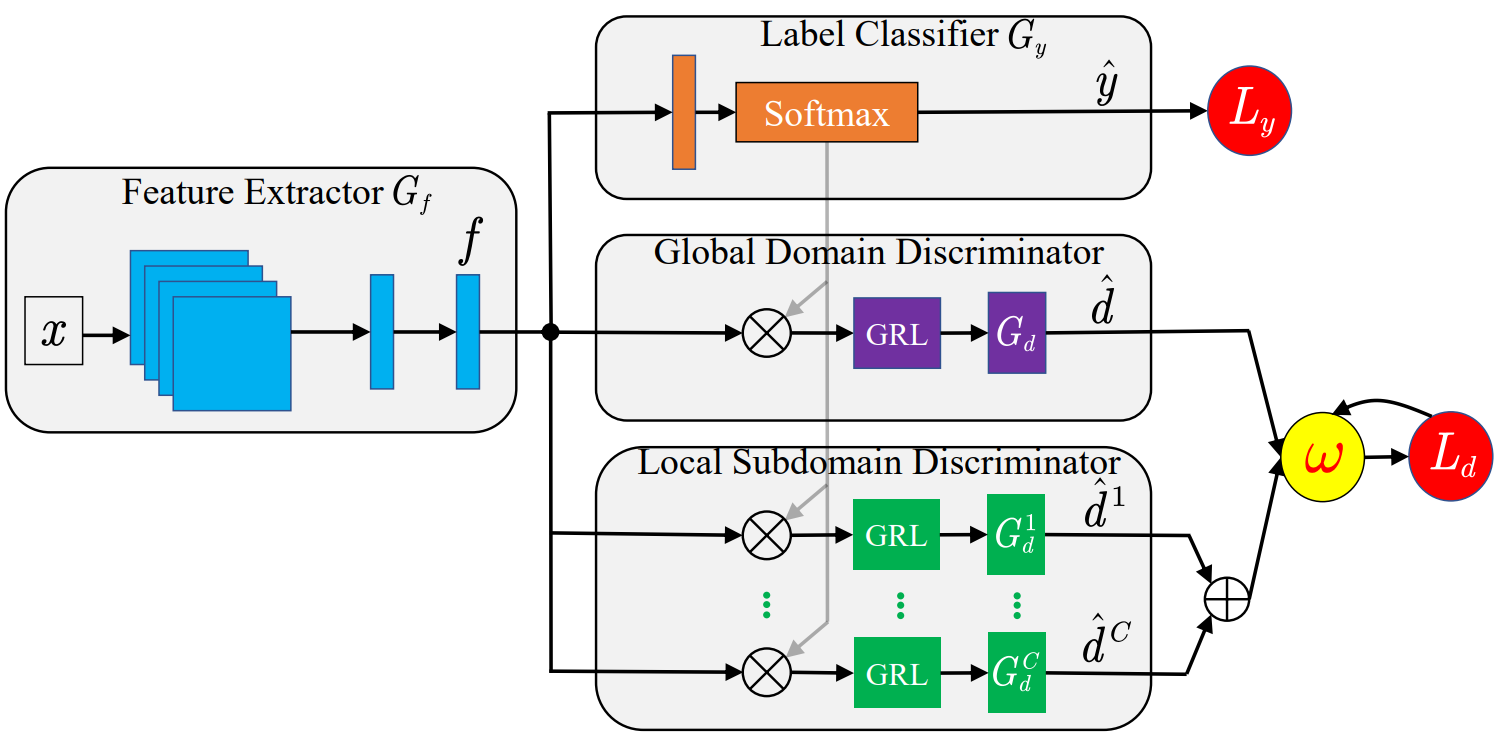
\includegraphics[scale=.35]{./figures/fig-distribution-daan.png}
	\caption{动态对抗适配网络DAAN结构示意图}
	\label{fig-daan}
\end{figure}

\subsection{小结}

综合上述三种概率分布自适应方法,我们可以得出如下的结论:

\begin{enumerate}
	\item 精度比较:DDA > JDA > TCA > 条件分布自适应。
	\item 将不同的概率分布自适应方法用于神经网络,是一个发展趋势。将概率分布适配加入深度网络中,往往会取得比非深度方法更好的结果。
\end{enumerate}

